% Options for packages loaded elsewhere
% Options for packages loaded elsewhere
\PassOptionsToPackage{unicode}{hyperref}
\PassOptionsToPackage{hyphens}{url}
\PassOptionsToPackage{dvipsnames,svgnames,x11names}{xcolor}
%
\documentclass[
  letterpaper,
  DIV=11,
  numbers=noendperiod]{scrartcl}
\usepackage{xcolor}
\usepackage{amsmath,amssymb}
\setcounter{secnumdepth}{-\maxdimen} % remove section numbering
\usepackage{iftex}
\ifPDFTeX
  \usepackage[T1]{fontenc}
  \usepackage[utf8]{inputenc}
  \usepackage{textcomp} % provide euro and other symbols
\else % if luatex or xetex
  \usepackage{unicode-math} % this also loads fontspec
  \defaultfontfeatures{Scale=MatchLowercase}
  \defaultfontfeatures[\rmfamily]{Ligatures=TeX,Scale=1}
\fi
\usepackage{lmodern}
\ifPDFTeX\else
  % xetex/luatex font selection
\fi
% Use upquote if available, for straight quotes in verbatim environments
\IfFileExists{upquote.sty}{\usepackage{upquote}}{}
\IfFileExists{microtype.sty}{% use microtype if available
  \usepackage[]{microtype}
  \UseMicrotypeSet[protrusion]{basicmath} % disable protrusion for tt fonts
}{}
\makeatletter
\@ifundefined{KOMAClassName}{% if non-KOMA class
  \IfFileExists{parskip.sty}{%
    \usepackage{parskip}
  }{% else
    \setlength{\parindent}{0pt}
    \setlength{\parskip}{6pt plus 2pt minus 1pt}}
}{% if KOMA class
  \KOMAoptions{parskip=half}}
\makeatother
% Make \paragraph and \subparagraph free-standing
\makeatletter
\ifx\paragraph\undefined\else
  \let\oldparagraph\paragraph
  \renewcommand{\paragraph}{
    \@ifstar
      \xxxParagraphStar
      \xxxParagraphNoStar
  }
  \newcommand{\xxxParagraphStar}[1]{\oldparagraph*{#1}\mbox{}}
  \newcommand{\xxxParagraphNoStar}[1]{\oldparagraph{#1}\mbox{}}
\fi
\ifx\subparagraph\undefined\else
  \let\oldsubparagraph\subparagraph
  \renewcommand{\subparagraph}{
    \@ifstar
      \xxxSubParagraphStar
      \xxxSubParagraphNoStar
  }
  \newcommand{\xxxSubParagraphStar}[1]{\oldsubparagraph*{#1}\mbox{}}
  \newcommand{\xxxSubParagraphNoStar}[1]{\oldsubparagraph{#1}\mbox{}}
\fi
\makeatother


\usepackage{longtable,booktabs,array}
\usepackage{calc} % for calculating minipage widths
% Correct order of tables after \paragraph or \subparagraph
\usepackage{etoolbox}
\makeatletter
\patchcmd\longtable{\par}{\if@noskipsec\mbox{}\fi\par}{}{}
\makeatother
% Allow footnotes in longtable head/foot
\IfFileExists{footnotehyper.sty}{\usepackage{footnotehyper}}{\usepackage{footnote}}
\makesavenoteenv{longtable}
\usepackage{graphicx}
\makeatletter
\newsavebox\pandoc@box
\newcommand*\pandocbounded[1]{% scales image to fit in text height/width
  \sbox\pandoc@box{#1}%
  \Gscale@div\@tempa{\textheight}{\dimexpr\ht\pandoc@box+\dp\pandoc@box\relax}%
  \Gscale@div\@tempb{\linewidth}{\wd\pandoc@box}%
  \ifdim\@tempb\p@<\@tempa\p@\let\@tempa\@tempb\fi% select the smaller of both
  \ifdim\@tempa\p@<\p@\scalebox{\@tempa}{\usebox\pandoc@box}%
  \else\usebox{\pandoc@box}%
  \fi%
}
% Set default figure placement to htbp
\def\fps@figure{htbp}
\makeatother


% definitions for citeproc citations
\NewDocumentCommand\citeproctext{}{}
\NewDocumentCommand\citeproc{mm}{%
  \begingroup\def\citeproctext{#2}\cite{#1}\endgroup}
\makeatletter
 % allow citations to break across lines
 \let\@cite@ofmt\@firstofone
 % avoid brackets around text for \cite:
 \def\@biblabel#1{}
 \def\@cite#1#2{{#1\if@tempswa , #2\fi}}
\makeatother
\newlength{\cslhangindent}
\setlength{\cslhangindent}{1.5em}
\newlength{\csllabelwidth}
\setlength{\csllabelwidth}{3em}
\newenvironment{CSLReferences}[2] % #1 hanging-indent, #2 entry-spacing
 {\begin{list}{}{%
  \setlength{\itemindent}{0pt}
  \setlength{\leftmargin}{0pt}
  \setlength{\parsep}{0pt}
  % turn on hanging indent if param 1 is 1
  \ifodd #1
   \setlength{\leftmargin}{\cslhangindent}
   \setlength{\itemindent}{-1\cslhangindent}
  \fi
  % set entry spacing
  \setlength{\itemsep}{#2\baselineskip}}}
 {\end{list}}
\usepackage{calc}
\newcommand{\CSLBlock}[1]{\hfill\break\parbox[t]{\linewidth}{\strut\ignorespaces#1\strut}}
\newcommand{\CSLLeftMargin}[1]{\parbox[t]{\csllabelwidth}{\strut#1\strut}}
\newcommand{\CSLRightInline}[1]{\parbox[t]{\linewidth - \csllabelwidth}{\strut#1\strut}}
\newcommand{\CSLIndent}[1]{\hspace{\cslhangindent}#1}



\setlength{\emergencystretch}{3em} % prevent overfull lines

\providecommand{\tightlist}{%
  \setlength{\itemsep}{0pt}\setlength{\parskip}{0pt}}



 


\usepackage{authblk}
\usepackage{orcidlink}
\usepackage{newunicodechar}
\newunicodechar{ʻ}{`}
\usepackage{xr}
\externaldocument{hawaii-arth-mete-supp}
\newcommand{\sfig}[1]{Supplementary Figure~\ref{#1}}
\newcommand{\ssec}[1]{Supplementary Section~\ref{#1}}
\renewcommand{\sfdefault}{\rmdefault}
\KOMAoption{captions}{tableheading}
\author[1]{Andrew J. Rominger\,\orcidlink{0000-0003-3755-4480}}
\author[1]{Katie Thai\,\orcidlink{0009-0006-1223-122X}}
\author[2]{Rosemary G. Gillespie\,\orcidlink{0000-0003-0086-7424}}
\author[3]{Daniel S. Gruner\,\orcidlink{0000-0002-3153-4297}}
\author[2]{John Harte\,\orcidlink{0000-0002-8794-5140}}
\affil[1]{University of Hawaiʻi at Mānoa}
\affil[2]{University of California Berkeley}
\affil[3]{University of Maryland}
\renewcommand*{\author}[2][]{}
\makeatletter
\@ifpackageloaded{caption}{}{\usepackage{caption}}
\AtBeginDocument{%
\ifdefined\contentsname
  \renewcommand*\contentsname{Table of contents}
\else
  \newcommand\contentsname{Table of contents}
\fi
\ifdefined\listfigurename
  \renewcommand*\listfigurename{List of Figures}
\else
  \newcommand\listfigurename{List of Figures}
\fi
\ifdefined\listtablename
  \renewcommand*\listtablename{List of Tables}
\else
  \newcommand\listtablename{List of Tables}
\fi
\ifdefined\figurename
  \renewcommand*\figurename{Figure}
\else
  \newcommand\figurename{Figure}
\fi
\ifdefined\tablename
  \renewcommand*\tablename{Table}
\else
  \newcommand\tablename{Table}
\fi
}
\@ifpackageloaded{float}{}{\usepackage{float}}
\floatstyle{ruled}
\@ifundefined{c@chapter}{\newfloat{codelisting}{h}{lop}}{\newfloat{codelisting}{h}{lop}[chapter]}
\floatname{codelisting}{Listing}
\newcommand*\listoflistings{\listof{codelisting}{List of Listings}}
\makeatother
\makeatletter
\makeatother
\makeatletter
\@ifpackageloaded{caption}{}{\usepackage{caption}}
\@ifpackageloaded{subcaption}{}{\usepackage{subcaption}}
\makeatother
\usepackage{bookmark}
\IfFileExists{xurl.sty}{\usepackage{xurl}}{} % add URL line breaks if available
\urlstyle{same}
\hypersetup{
  pdftitle={Eco-evolutionary deviations from steady state across the Hawaiian chronosequence revealed with a maximum entropy perspective},
  colorlinks=true,
  linkcolor={blue},
  filecolor={Maroon},
  citecolor={Blue},
  urlcolor={Blue},
  pdfcreator={LaTeX via pandoc}}


\title{Eco-evolutionary deviations from steady state across the Hawaiian
chronosequence revealed with a maximum entropy perspective}
\author{}
\date{}
\begin{document}
\maketitle


\subsection{Introduction}\label{introduction}

Biodiversity patterns are bound by two seemingly contradictory states:
they show striking consistency in form across systems, and yet also must
emerge in spite of, or because of, the constant flux and dynamic change
of ecology and evolution. The near universality of biodiversity patterns
includes the scaling of species richness with area, the ubiquity of rare
spaces and scarcity of common species, and the highly skewed
distribution of biomass or metabolic resource use across organisms.
Debate has persisted for over a century as to whether these consistent
patterns form because of ecological and evolutionary drivers that force
systems into these configurations, or are largely the outcome of chance
acting on large systems of constituent parts. The former gives rise to
niche-based theories of coexistence, while that later has produced a
number of neutral-like models.

Both deterministic and stochastic perspectives on the generation of
universal biodiversity patterns most often make the choice of
considering an ecosystem at ``equilibrium'' or steady state. However,
ecosystems are known to be dynamic both through intrinsic
eco-evolutionary processes and due to recent anthropogenic perturbation.
Whether universal patterns are insensitive to non-steady-state processes
or are a result of those processes remains addressed. To better
understand the interaction of non-steady-state processes and universal
patterns, we combine data from the highly dynamic ecosystems of the
Hawaiian Archipelago with the intentionally minimalist steady state
predictions of the Maximum Entropy Theory of Ecology.

\subsubsection{The Hawaiian
Chronosequence}\label{the-hawaiian-chronosequence}

The Hawaiian Archipelago holds numerous examples of adaptive radiation
(Baldwin \& Sanderson 1998; Bennett \& O'Grady 2013; Gillespie 2004;
Givnish \emph{et al.} 2009; Knope \emph{et al.} 2012; Lerner \emph{et
al.} 2011; Magnacca \& Price 2015). Those remarkable examples of
diversification along with the geographic isolation and chronological
geology of the archipelago have made it a focal point for the study of
eco-evolutionary processes (Barton \emph{et al.} 2021; Chadwick \emph{et
al.} 1999; Gillespie \& Clague 2009; Price \& Wagner 2004; Simon 1987;
Wagner \& Funk 1995). The manner in which the islands formed in
chronological sequence Figure~\ref{fig-chrono} has allowed for the study
of ecosystems in different stages of eco-evolutionary assembly
(Gillespie 2004; Rominger \emph{et al.} 2016; Vitousek 2004) by
considering ecosystems on different aged substrates to be snapshots of
eco-evolutionary processes at different time points.

\begin{figure}

\centering{

\pandocbounded{\includegraphics[keepaspectratio]{hawaii-arth-mete_files/figure-pdf/fig-chrono-1.pdf}}

}

\caption{\label{fig-chrono}Chronosequence of the Hawaiian Archipelago
showing oldest flows to the west on Kauaʻi and youngest flows to the
east on Hawaiʻi. Substrate age data from Sherrod \emph{et al.} (2021).
The five sites are indicated with dots on the map and arrows indicating
their flow ages on the legend. From oldest to youngest (west to east)
sites are: Alakaʻi, Kamakou, Kohala, Laupāhoehoe, Kīlauea.}

\end{figure}%

Hawaiʻi has also been subjected to pervasive anthropogenic changes to
its biodiversity, especially a rapidly expanded human land-use footprint
and markedly accelerated introduction of non-native species following
Western contact and settler colonialism (Gon \emph{et al.} 2018; Graham
\emph{et al.} 2017). As such Hawaiʻi has produced numerous studies of
rare and endangered species (Magnacca 2007; Pratt \emph{et al.} 2009;
Régnier \emph{et al.} 2015; Sakai \emph{et al.} 2002) and the functions
of non-native species in ecosystems (Barton \emph{et al.} 2021; Ostertag
\emph{et al.} 2009).

Arthropods in Hawaiʻi represent both many adaptive radiations (Bennett
\& O'Grady 2013; Gillespie 2004; Magnacca \& Price 2015), many rare
species (Magnacca 2007; Magnacca \& Price 2015), and many introduced
species (Nishida 1992). Given their abundance and diversity, they also
present a unique opportunity to use ecological theory to study how
biodiversity conforms to or deviates from steady state.

\subsubsection{The Maximum Entropy Theory of
Ecology}\label{the-maximum-entropy-theory-of-ecology}

The Maximum Entropy Theory of Ecology (METE Harte (2011)) is a
particularly useful tool for studying steady state biodiversity patterns
because it produces multiple testable predictions, making falsifications
of the theory more informative (McGill 2003) including the distribution
of abundances across species and the distribution of metabolic rates
across individuals in a sample. METE arrives at some similar predictions
to other null or neutral models of biodiversity such at the Unified
Neutral Theory (Hubbell 2001) but instead of being limited to a single
neutral formulation, METE is grounded in the principles of statistical
mechanics Jaynes (1957) drawing from the probabilistic properties of
large, randomly assembled systems. Thus its predictions represent a
community in statistical steady state. Statistical steady state means
that a system is governed by only a few simple state variables, which
constitute a state space, and that no additional processes limit the
system's ability to freely explore this state space. The state variables
of METE are total number of species \(S_0\), total number of individuals
\(N_0\), and summed metabolic rate across all individuals \(E_0\) (Harte
2011). METE posits that if state variables are in steady state, all
biodiversity patterns are statistical outcomes from those state
variables independently of the specific biological mechanisms governing
the values of the state variables, so long as those mechanisms do not
constitute information beyond the state variables themselves. Examples
of such additional information could be rapid environmental change
leading to mismatched niches with local environments, rapid
diversification, or biological invasion. Under such scenarios the simple
state variables of \(S_0\), \(N_0\), and \(E_0\) would not likely
constitute enough information to yield accurate predictions for
biodiversity patterns such as the species abundance distribution or
distribution of metabolic rates across individuals. Thus finding
deviations between observed patterns of abundance and metabolic rate
distributions compared to their METE predictions allows us to identify
ecological systems out of statistical steady state (Harte 2011; Newman
\emph{et al.} 2020; Rominger \emph{et al.} 2016).

In this study of arthropods communities across the Hawaiian
chronosequence, we find consistent deviations from steady state at
middle aged sites. Deviations are predicted by community dissimilarity
which peaks at middle aged sites. This suggests these communities are
unstable, perhaps due to their age being the right time for adaptive
radiation to take off for arthropods (Bennett \& O'Grady 2013; Gillespie
2004). Deviations are also partially predicted by proportion of
non-native species, except that the proportion of non-native species is
high at the youngest site while this site also shows some of the lowest
deviations from METE. This suggests the role of biological invasion is
context dependent, at times producing stead state and at others driving
deviation from it. More work connecting deviations from steady state to
ecological and evolutionary drivers will be needed to further test these
possibilities.

\subsection{Methods}\label{methods}

\subsubsection{Reproducibility and data
preparation}\label{reproducibility-and-data-preparation}

A custom R package, \emph{HawaiiArthMETE} (Rominger \& Thai 2026),
accompanies this paper and can be used to reproduce all results. All
data analyzed here are available via the package as described in
\ssec{sec-setup}.

Arthropod data come from the original publication by Gruner (2007), a
study that collected 17024 specimens across the Hawaiian chronosequence
Figure~\ref{fig-chrono}. Study sites in Gruner (2007) where standardized
to be climatically homogeneous, seeking to capture differences in
arthropod assemblages due to substrate age and not other abiotic
factors.

Each specimen was identified to the species level (morpho species were
used in 31.56\% of specimens). Specimen lengths were measured to the
nearest millimeter. For METE analyses we need to estimate metabolic rate
from these data. Because METE normalizes metabolic rates such that the
lowest possible rate is 1 we use a simplified \(3/4\) scaling rule to
approximate metabolic rate \(B\) from mass \(M\) as
\(B \propto M^{3/4}\).

This leaves the estimation of mass from length. Gruner (2007) used
taxon- and stage- specific length-to-biomass allometric scaling
relationships (Gruner 2003) to approximate mass as the expected value of
a log-log regression

\[
\begin{aligned}
\text{mass} & = e^{\widehat{\log(\text{mass})}} \\
\widehat{\log(\text{mass})} &= \log(a) + b \cdot \log(\text{length})
\end{aligned}
\]

where \(a\) and \(b\) are estimated from data collected by Gruner (2003)
and vary by taxon and stage.

Using these expected value masses based on length measured to the
nearest milliliter yields metabolic rate approximations that are
artificially discretization (see the appendix ``Sampling biomass
estimates from allometric equations''). These descretizations in turn
lead to spurious conclusions about the predicitiveness of METE because
METE assumes metabolic rates are continuous (see \ssec{sec-re-run}).

Therefore, instead of estimating mass as the expected value from an
allometric relationship we sample masses as random draws from the full
model relating mass to length

\[
\begin{aligned}
\text{mass} & = e^{y} \\
y &\sim \mathscr{N}(\widehat{\log(\text{mass})}, ~\sigma) \\
\widehat{\log(\text{mass})} &= \log(a) + b \cdot \log(\text{length})
\end{aligned}
\]

where \(\sigma\) is the taxon- and stage-specific standard deviation of
residuals. The full procedure for sampling masses is detailed in the
appendix ``Sampling biomass estimates from allometric equations'' and
the consequences of using random draws versus expected values on the
METE analysis is thoroughly investigated in \ssec{sec-re-run}. We
conclude that using random draws for mass estimates is largely similar
to using expected values, and our overall conclusions are unchanged, but
using draws avoids both spurious deviations from and conformations to
METE that would be introduced by using expected values of mass.

\subsubsection{METE analysis}\label{mete-analysis}

To produce METE predictions for the SAD and IPD we use the \emph{meteR}
R package (Rominger \& Merow 2017). We compare these predictions to
observed SAD and IPD patterns using a \(z^2\)-value. The use of
\(z^2\)-values is discussed in Rominger \& Merow (2017), but briefly:
the \(z^2\)-value compares the log likelihood of the data given them
METE model to the log likelihood of a hypothetical data set drawn from
the METE model itself. This comparison is done many times and the actual
\(z^2\)-value is calculated as

\[
z^2 = \left(\frac{\log(\mathscr{L}(\text{data} \mid \text{METE})) - \hat{\mu}_{\log\mathscr{L}_\text{METE}}}{\hat{\sigma}_{\log\mathscr{L}_\text{METE}}}\right)^2
\]

where \(\hat{\mu}_{\log\mathscr{L}_\text{METE}}\) is the mean of the log
likelihood of data drawn from METE itself, and
\(\hat{\sigma}_{\log\mathscr{L}_\text{METE}}\) is the standard deviation
of the log likelihood of data drawn from METE itself.

If METE is truly correct in describing the data, \(z^2\) will
asymptotically have a \(\chi^2\) distribution with \(d.f. = 1\)
(Rominger \& Merow 2017). If METE does not truly describe the data, the
\(z^2\)-value is likely to be large.

We also quantify the difference between METE predictions and observed
SADs and IPDs by comparing the tails of the observed and predicted
distributions. These tails can be especially informative about the
nature of deviations (Harte 2011). For the SAD we compare rarity as the
log ratio of observed proportion of singletons to the predicted
proportion of singletons, and we compare dominance as log ration of
observed total abundance of the top three most abundant species to the
predicted total abundance of the top three most abundant species. For
the IPD we compare metrics similar to rarity and dominance: the log
ratio of observed proportion of individuals with a scaled metabolism of
less than 3 to its prediction, and the log ratio of the observed sum of
metabolic rates for the top 10 individuals to its prediction.

\subsection{Statistical analysis of deviations from METE and potential
explanatory
variables}\label{statistical-analysis-of-deviations-from-mete-and-potential-explanatory-variables}

We first evaluate how deviations from METE, as measured by
\(z^2\)-values, vary across the chronosequence. We then test for
relationships between \(z^2\)-values and proportion of non-native
species at a site as well as within site, between sample dissimilarity
or \(\beta\)-diversity.

For all these analyses we fit linear models predicting log-transformed
\(z^2\)-values responding to each explanatory variable: substrate age,
proportion non-native species, and within site \(\beta\)-diversity.
Log-transforming \(z^2\)-values brings them closer to the normal
assumptions of a linear model. The need for log-transformation is not
surprising: while \(z^2\)-values will be \(\chi^2\) distributed if METE
is true, deviations from METE add more probability to larger values, and
taken together will lead to right-skewed distribution of \(z^2\)-values.
Log-transformation brings right-skewed random variables closer to
normal.

When modeling deviations from METE, we have two statistical challenges
to address: samples within sites could represent pseudo replicates
necessitating a random-effects model; however, because explanatory
variables are site-level characteristics, site-level random effects
would be completely collinear with site-level explanatory variables.

To address these challenges we model the site-level mean and variance
rather than each individual sample within each site. This is the most
conservative approach but runs the risk of being under-powered because
while we have 48 samples, we only have 5 sites. Modeling mean and
variance is the same technique used in meta-analyses. We therefore make
use of the \emph{metafor} package (Viechtbauer 2010) in fitting testing
these models.

\subsection{\texorpdfstring{Calculating
\(\beta\)-diversity}{Calculating \textbackslash beta-diversity}}\label{calculating-beta-diversity}

To quantify within site, between sample \(\beta\)-diversity we first
calculate mean Bray-Curtis dissimilarity between samples and then, to
standardize \(\beta\)-diversity measures across sites, we normalize mean
dissimilarity to a null model. We use the \texttt{quasiswap\_count}
algorithm implemented in \emph{vegan} (Oksanen \emph{et al.} 2025) to
generate null samples. This algorithm preserves row and column sums of a
sample by species matrix and also seeks to maintain null matrix fill
close to the observed fill thereby mimicking patchiness in the real
data. We use 500 null sample by species matrices to generate null models
for each site. Then normalized within site, between sample
\(\beta\)-diversity was calculated as a z-score

\[
\text{Normalized }\beta = \frac{\text{BC}_\text{obs} - \mu_\text{null}}{\sigma_\text{null}}
\]

where \(BC_\text{obs}\) is the observed mean Bray-Curtis dissimilarity
between samples within a site, \(\mu_\text{null}\) is the mean of the
null distribution, and \(\sigma_\text{null}\) is the standard deviation
of the null distribution.

We are also interested in understanding how native and non-native
species contribute to the overall mean dissimilarity at a site. We can
do this by partitioning Bray Curtis dissimilarity between native and
non-native groups of species. \ssec{sec-part} provides the mathematical
and computational details of how we do this. The end result of
partitioning Bray-Curtis dissimilarity between native and non-native
species is that we have a ratio of within site \(\beta\)-diversity
attributable to native species to that attributable to non-native
species. We take the log of this ratio such that equal contributions of
native and non-native species yields a log ratio of 0.

We also compare this Bray Curtis dissimilarity partitioning to a null
model. Here the \texttt{quasiswap\_count} algorithm will not work
because it permutes individuals across species as well as sites. Instead
we want to only shuffle the label of each species: native or non-native.
But we still need to maintain, at least probabilistically, attributes of
the data that might confound null model analysis. Specifically, we
should seek to maintain, in probability, the distribution of abundances
of native and non-native species. We wrote a custom algorithm to do this
in the \emph{HawaiiArthMETE} package and described in \ssec{sec-bart}.

\subsection{Results}\label{results}

\subsubsection{Deviations from METE across the
chronosequence}\label{deviations-from-mete-across-the-chronosequence}

\begin{figure}

\centering{

\pandocbounded{
\includegraphics[keepaspectratio]{hawaii-arth-mete_files/figure-pdf/fig-z2-chrono-1.pdf}}

}

\caption{\label{fig-z2-chrono}Deviations from METE across the
chronosequence as measured by \(z^2\)-values. Colors represent sites and
match the color coding of substrate age in Figure~\ref{fig-chrono}.}

\end{figure}%

Deviations from METE in the SAD an IPD both peak at middle aged sites
along the chronosequence Figure~\ref{fig-z2-chrono}. This is supported
by a likelihood ratio test comparing a quadratic model of \(z^2\)-values
to an intercept-only model. For SAD \(z^2\)-values the LRT statistic is
\(\Lambda =\) 28.7299696 with \(d.f. =\) 2 and \(P\) \textless{} 0.0001.
For IPD \(z^2\)-values the LRT statistic is \(\Lambda =\) 5.5130141 with
\(d.f. =\) 2 and \(P\) = 0.0635.

\begin{verbatim}
$QM
[1] 28.72997

$QMdf
[1]  2 NA

$QMp
[1] 5.772532e-07

$btt
[1] 2 3

$k
[1] 5

$p
[1] 3

$m
[1] 2

$test
[1] "z"

$digits
  est    se  test  pval    ci   var sevar   fit   het 
    4     4     4     4     4     4     4     4     4 

$type
[1] "Wald.btt"

$class
[1] "rma.uni" "rma"    

attr(,"class")
[1] "anova.rma"
\end{verbatim}

\begin{itemize}
\tightlist
\item
  deviations for SAD and IPD peak at middle age
\item
  deviations for IPD larger overall
\item
  deviations of SAD are because of more unevenness (more singletons and
  more hyper abundant species)
\item
  no consistent relationship between IDP deviations and the extremes of
  the distribution (deviation is in the middle)
\end{itemize}

\begin{figure}

\centering{

\pandocbounded{
\includegraphics[keepaspectratio]{hawaii-arth-mete_files/figure-pdf/fig-how-z2-1.pdf}}

}

\caption{\label{fig-how-z2}Relationship between \(z^2\) measure of
deviation from METE and different metrics describing how observed data
and METE predictions diverge.}

\end{figure}%

\subsection{\texorpdfstring{Deviations from METE predicted by non-native
species and
\(\beta\)-diversity}{Deviations from METE predicted by non-native species and \textbackslash beta-diversity}}\label{deviations-from-mete-predicted-by-non-native-species-and-beta-diversity}

\begin{figure}

\centering{

\pandocbounded{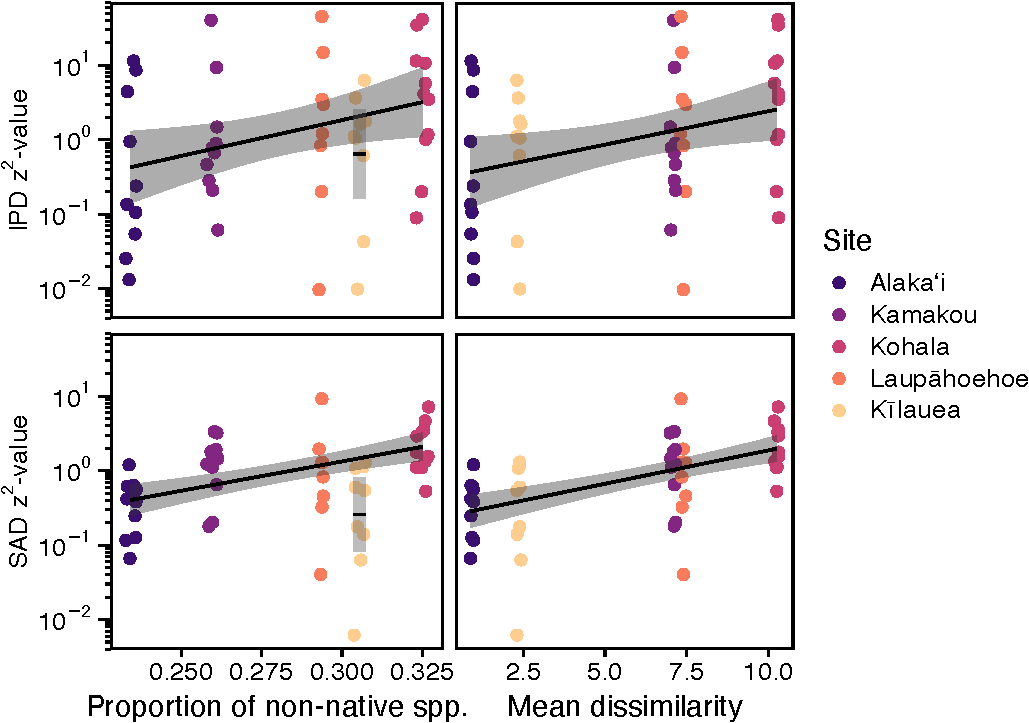
\includegraphics[keepaspectratio]{hawaii-arth-mete_files/figure-pdf/fig-pred-1.pdf}}

}

\caption{\label{fig-pred}Relationship between \(z^2\) measure of
deviation from METE and different predictor variables: proportion of
non-native species and \(\beta\)-diversity.}

\end{figure}%

\begin{itemize}
\tightlist
\item
  deviations are predicted by proportion of non-natives
\item
  deviations are predicted by dissimilarity
\end{itemize}

\subsection{\texorpdfstring{Partitioning \(\beta\)-diversity across
native and non-native
species}{Partitioning \textbackslash beta-diversity across native and non-native species}}\label{partitioning-beta-diversity-across-native-and-non-native-species}

\begin{figure}

\centering{

\pandocbounded{
\includegraphics[keepaspectratio]{hawaii-arth-mete_files/figure-pdf/fig-bray-part-1.pdf}}

}

\caption{\label{fig-bray-part}Difference in contribution of native and
non-native species to dissimilarity compared to null. Negative values
indicate greater contribution of non-native species compared to chance
while positive values indicate greater contribution of native species
compared to chance.}

\end{figure}%

\begin{itemize}
\tightlist
\item
  something is going on at Kīlauea
\end{itemize}

\subsection{Discussion}\label{discussion}

\begin{itemize}
\tightlist
\item
  dissimilarity as instability
\item
  possible causes of instability---adaptive radiation
\item
  presents future hypothesis to test with genetic data
\item
  hypotheses

  \begin{itemize}
  \tightlist
  \item
    diversification drives divergence; diversification slowed down on
    older flows
  \item
    invasion drives divergence
  \item
    both do and they interact, perhaps even conditions favoring
    diversification favor invasion too
  \end{itemize}
\end{itemize}

\subsection*{References}\label{references}
\addcontentsline{toc}{subsection}{References}

\phantomsection\label{refs}
\begin{CSLReferences}{1}{0}
\bibitem[\citeproctext]{ref-baldwin1998}
Baldwin, B.G. \& Sanderson, M.J. (1998).
\href{https://doi.org/10.1073/pnas.95.16.9402}{Age and rate of
diversification of the {Hawaiian} silversword alliance ({Compositae})}.
\emph{Proceedings of the National Academy of Sciences}, 95, 9402--9406.

\bibitem[\citeproctext]{ref-barton2021}
Barton, K.E., Westerband, A., Ostertag, R., Stacy, E., Winter, K.,
Drake, D.R., \emph{et al.} (2021).
\href{https://doi.org/10.1016/j.ppees.2021.125631}{{Hawai`i} forest
review: Synthesizing the ecology, evolution, and conservation of a model
system}. \emph{Perspectives in Plant Ecology, Evolution and
Systematics}, 52, 125631.

\bibitem[\citeproctext]{ref-bennett2013}
Bennett, G.M. \& O'Grady, P.M. (2013). Historical biogeography and
ecological opportunity in the adaptive radiation of native hawaiian
leafhoppers (cicadellidae: nesophrosyne). \emph{Journal of
Biogeography}, 40, 1512--1523.

\bibitem[\citeproctext]{ref-chadwick1999}
Chadwick, O.A., Derry, L.A., Vitousek, P.M., Huebert, B.J. \& Hedin,
L.O. (1999). Changing sources of nutrients during four million years of
ecosystem development. \emph{Nature}, 397, 491--497.

\bibitem[\citeproctext]{ref-gillespie2004}
Gillespie, R.G. (2004).
\href{https://doi.org/10.1126/science.1091875}{Community assembly
through adaptive radiation in {Hawaiian} spiders}. \emph{Science}, 303,
356--359.

\bibitem[\citeproctext]{ref-gillespie_clague2009}
Gillespie, R.G. \& Clague, D.A. (2009). \emph{Encyclopedia of islands}.
Univ of California Press.

\bibitem[\citeproctext]{ref-givnish2009}
Givnish, T.J., Millam, K.C., Mast, A.R., Paterson, T.B., Theim, T.J.,
Hipp, A.L., \emph{et al.} (2009).
\href{https://doi.org/10.1098/rspb.2008.1204}{Origin, adaptive radiation
and diversification of the {Hawaiian} lobeliads ({Asterales}:
{Campanulaceae})}. \emph{Proceedings of the Royal Society B: Biological
Sciences}, 276, 407--416.

\bibitem[\citeproctext]{ref-gon2018}
Gon, S.M., Tom, S.L. \& Woodside, U. (2018).
\href{https://doi.org/10.3390/su10103420}{`Āina momona, honua au
loli---{Productive} lands, changing world: Using the {Hawaiian}
footprint to inform biocultural restoration and future sustainability in
{Hawai`i}}. \emph{Sustainability}, 10, 3420.

\bibitem[\citeproctext]{ref-graham2017}
Graham, N.R., Gruner, D.S., Lim, J.Y. \& Gillespie, R.G. (2017). Island
ecology and evolution: Challenges in the anthropocene.
\emph{Environmental Conservation}, 44, 323--335.

\bibitem[\citeproctext]{ref-gruner2003}
Gruner, D.S. (2003). Regressions of length and width to predict
arthropod biomass in the hawaiian islands. \emph{Pacific Science}, 57,
325--336.

\bibitem[\citeproctext]{ref-gruner2007}
Gruner, D.S. (2007). Geological age, ecosystem development, and local
resource constraints on arthropod community structure in the hawaiian
islands. \emph{Biological Journal of the Linnean Society}, 90, 551--570.

\bibitem[\citeproctext]{ref-harte2011}
Harte, J. (2011). \emph{Maximum entropy and ecology: A theory of
abundance, distribution, and energetics}. OUP Oxford.

\bibitem[\citeproctext]{ref-hubbell2001}
Hubbell, S.P. (2001). \emph{The unified neutral theory of biodiversity
and biogeography (MPB-32)}. Princeton University Press.

\bibitem[\citeproctext]{ref-jaynes1957}
Jaynes, E. (1957). {Information theory and statistical mechanics. II}.
\emph{Physical Review}, 108, 171--190.

\bibitem[\citeproctext]{ref-knope2012}
Knope, M.L., Morden, C.W., Funk, V.A. \& Fukami, T. (2012).
\href{https://doi.org/10.1111/j.1365-2699.2012.02687.x}{Area and the
rapid radiation of {Hawaiian} \emph{bidens} ({Asteraceae})}.
\emph{Journal of Biogeography}, 39, 1206--1216.

\bibitem[\citeproctext]{ref-lerner2011}
Lerner, H.R.L., Meyer, M., James, H.F., Hofreiter, M. \& Fleischer, R.C.
(2011). \href{https://doi.org/10.1016/j.cub.2011.09.039}{Multilocus
resolution of phylogeny and timescale in the extant adaptive radiation
of {Hawaiian} honeycreepers}. \emph{Current Biology}, 21, 1838--1844.

\bibitem[\citeproctext]{ref-magnacca2007}
Magnacca, K.N. (2007).
\href{https://doi.org/10.2984/1534-6188(2007)61\%5B173:CSOTEB\%5D2.0.CO;2}{Conservation
status of the endemic bees of {Hawai`i}, \emph{hylaeus}
(\emph{nesoprosopis}) ({Hymenoptera}: {Colletidae})}. \emph{Pacific
Science}, 61, 173--190.

\bibitem[\citeproctext]{ref-magnacca2015}
Magnacca, K.N. \& Price, D.K. (2015).
\href{https://doi.org/10.1016/j.ympev.2015.06.014}{Rapid adaptive
radiation and host plant conservation in the {Hawaiian} picture wing
\emph{drosophila} ({Diptera}: {Drosophilidae})}. \emph{Molecular
Phylogenetics and Evolution}, 92, 226--242.

\bibitem[\citeproctext]{ref-mcgill2003}
McGill, B. (2003). Strong and weak tests of macroecological theory.
\emph{Oikos}, 102, 679--685.

\bibitem[\citeproctext]{ref-newman2020}
Newman, E.A., Wilber, M.Q., Kopper, K.E., Moritz, M.A., Falk, D.A.,
McKenzie, D., \emph{et al.} (2020). Disturbance macroecology: A
comparative study of community structure metrics in a high-severity
disturbance regime. \emph{Ecosphere}, 11, e03022.

\bibitem[\citeproctext]{ref-hichecklist}
Nishida, G.M. (1992). \emph{Hawaiian terrestrial arthropod checklist}.
Bishop University Press, Honolulu.

\bibitem[\citeproctext]{ref-vegan}
Oksanen, J., Simpson, G.L., Blanchet, F.G., Kindt, R., Legendre, P.,
Minchin, P.R., \emph{et al.} (2025).
\emph{\href{https://doi.org/10.32614/CRAN.package.vegan}{Vegan:
Community ecology package}}.

\bibitem[\citeproctext]{ref-ostertag2009}
Ostertag, R., Cordell, S., Michaud, J., Cole, T.C., Schulten, J.R.,
Publico, K.M., \emph{et al.} (2009). Ecosystem and restoration
consequences of invasive woody species in a wet {Hawaiian} forest.
\emph{Ecosystems}, 12, 503--515.

\bibitem[\citeproctext]{ref-pratt2009}
Pratt, T.K., Atkinson, C.T., Banko, P.C., Jacobi, J.D. \& Woodworth,
B.L. (Eds.). (2009). \emph{Conservation biology of {Hawaiian} forest
birds: Implications for island avifauna}. Yale University Press, New
Haven, CT.

\bibitem[\citeproctext]{ref-price2004}
Price, J.P. \& Wagner, W.L. (2004). Speciation in hawaiian angiosperm
lineages: Cause, consequence, and mode. \emph{Evolution}, 58,
2185--2200.

\bibitem[\citeproctext]{ref-regnieretal2015}
Régnier, C., Achaz, G., Lambert, A., Cowie, R.H., Bouchet, P. \&
Fontaine, B. (2015). \href{https://doi.org/10.1073/pnas.1502350112}{Mass
extinction in poorly known taxa}. \emph{Proceedings of the National
Academy of Sciences}, 112, 7761--7766.

\bibitem[\citeproctext]{ref-rominger2016}
Rominger, A.J., Goodman, K.R., Lim, J.Y., Armstrong, E.E., Becking,
L.E., Bennett, G.M., \emph{et al.} (2016).
\href{https://doi.org/10.1111/geb.12341}{Community assembly on isolated
islands: Macroecology meets evolution}. \emph{Global Ecology and
Biogeography}, 25, 769--780.

\bibitem[\citeproctext]{ref-rominger-merow2016}
Rominger, A.J. \& Merow, C. (2017). meteR: An r package for testing the
maximum entropy theory of ecology. \emph{Methods in Ecology and
Evolution}, 8, 241--247.

\bibitem[\citeproctext]{ref-HawaiiArthMETE}
Rominger, A. \& Thai, K. (2026).
\href{https://doi.org/10.5281/zenodo.20319088}{{HawaiiArthMETE}}.

\bibitem[\citeproctext]{ref-sakai2002}
Sakai, A.K., Wagner, W.L. \& Mehrhoff, L.A. (2002).
\href{https://doi.org/10.1080/10635150252899770}{Patterns of
endangerment in the {Hawaiian} flora}. \emph{Systematic Biology}, 51,
276--302.

\bibitem[\citeproctext]{ref-sherrod2021}
Sherrod, D.R., Sinton, J.M., Sarah, W.E., Kelly, B.M. \& Robinson, J.E.
(2021). Geologic map database to accompany geologic map of the state of
hawaii. \emph{US Geological Survey (USGS) Data Release}, 1112.

\bibitem[\citeproctext]{ref-simon1987}
Simon, C. (1987). Hawaiian evolutionary biology: An introduction.
\emph{Trends in ecology \& evolution}, 2, 175--178.

\bibitem[\citeproctext]{ref-metafor}
Viechtbauer, W. (2010).
\href{https://doi.org/10.18637/jss.v036.i03}{Conducting meta-analyses in
{R} with the {metafor} package}. \emph{Journal of Statistical Software},
36, 1--48.

\bibitem[\citeproctext]{ref-vitusek2004}
Vitousek, P.M. (2004). \emph{Nutrient cycling and limitation: {Hawai`i}
as a model system}. Princeton University Press, Princeton, NJ.

\bibitem[\citeproctext]{ref-wagner-funk1995}
Wagner, W.L. \& Funk, V.A. (1995). \emph{Hawaiian biogeography:
Evolution on a hot spot archipelago}.

\end{CSLReferences}




\end{document}
